\documentclass[14pt]{extbook}
\usepackage{multicol, enumerate, enumitem, hyperref, color, soul, setspace, parskip, fancyhdr} %General Packages
\usepackage{amssymb, amsthm, amsmath, latexsym, units, mathtools} %Math Packages
\everymath{\displaystyle} %All math in Display Style
% Packages with additional options
\usepackage[headsep=0.5cm,headheight=12pt, left=1 in,right= 1 in,top= 1 in,bottom= 1 in]{geometry}
\usepackage[usenames,dvipsnames]{xcolor}
\usepackage{dashrule}  % Package to use the command below to create lines between items
\newcommand{\litem}[1]{\item#1\hspace*{-1cm}\rule{\textwidth}{0.4pt}}
\pagestyle{fancy}
\lhead{Progress Quiz 7}
\chead{}
\rhead{Version A}
\lfoot{3510-5252}
\cfoot{}
\rfoot{Summer C 2021}
\begin{document}

\begin{enumerate}
\litem{
Determine the vertical asymptotes and holes in the rational function below.\[ f(x) = \frac{12x^{3} -25 x^{2} -18 x + 40}{16x^{2} +32 x + 15} \]\begin{enumerate}[label=\Alph*.]
\item \( \text{Holes at } x = -0.75 \text{ and } x = -1.25 \text{ with no vertical asymptotes.} \)
\item \( \text{Vertical Asymptote of } x = 0.75 \text{ and hole at } x = -1.25 \)
\item \( \text{Vertical Asymptotes of } x = -0.75 \text{ and } x = -1.25 \text{ with no holes.} \)
\item \( \text{Vertical Asymptote of } x = -0.75 \text{ and hole at } x = -1.25 \)
\item \( \text{Vertical Asymptotes of } x = -0.75 \text{ and } x = 1.333 \text{ with a hole at } x = -1.25 \)

\end{enumerate} }
\litem{
Determine the vertical asymptotes and holes in the rational function below.\[ f(x) = \frac{9x^{3} -12 x^{2} -20 x + 16}{9x^{2} -18 x + 8} \]\begin{enumerate}[label=\Alph*.]
\item \( \text{Vertical Asymptote of } x = 1.333 \text{ and hole at } x = 0.667 \)
\item \( \text{Holes at } x = 1.333 \text{ and } x = 0.667 \text{ with no vertical asymptotes.} \)
\item \( \text{Vertical Asymptotes of } x = 1.333 \text{ and } x = 0.667 \text{ with no holes.} \)
\item \( \text{Vertical Asymptotes of } x = 1.333 \text{ and } x = -1.333 \text{ with a hole at } x = 0.667 \)
\item \( \text{Vertical Asymptote of } x = 1.0 \text{ and hole at } x = 0.667 \)

\end{enumerate} }
\litem{
Which of the following functions \textit{could} be the graph below?
\begin{center}
    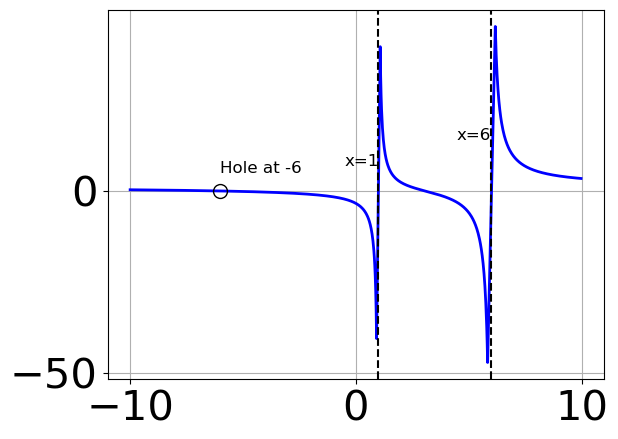
\includegraphics[width=0.5\textwidth]{../Figures/identifyGraphOfRationalFunctionCopyA.png}
\end{center}
\begin{enumerate}[label=\Alph*.]
\item \( f(x)=\frac{x^{3} -37.0 x -84.0}{x^{3} + x^{2} -36.0 x -36.0} \)
\item \( f(x)=\frac{x^{3} -37.0 x + 84.0}{x^{3} -1.0 x^{2} -36.0 x + 36.0} \)
\item \( f(x)=\frac{x^{3} +10.0 x^{2} +3.0 x -126.0}{x^{3} -1.0 x^{2} -36.0 x + 36.0} \)
\item \( f(x)=\frac{x^{3} -10.0 x^{2} +3.0 x + 126.0}{x^{3} + x^{2} -36.0 x -36.0} \)
\item \( \text{None of the above are possible equations for the graph.} \)

\end{enumerate} }
\litem{
Determine the horizontal and/or oblique asymptotes in the rational function below.\[ f(x) = \frac{3x^{2} +16 x + 16}{9x^{3} -36 x^{2} -16 x + 64} \]\begin{enumerate}[label=\Alph*.]
\item \( \text{Oblique Asymptote of } y = 3x -28. \)
\item \( \text{Horizontal Asymptote of } y = 0.333 \text{ and Oblique Asymptote of } y = 3x -28 \)
\item \( \text{Horizontal Asymptote at } y = -4.000 \)
\item \( \text{Horizontal Asymptote of } y = 0 \)
\item \( \text{Horizontal Asymptote of } y = 0.333  \)

\end{enumerate} }
\litem{
Which of the following functions \textit{could} be the graph below?
\begin{center}
    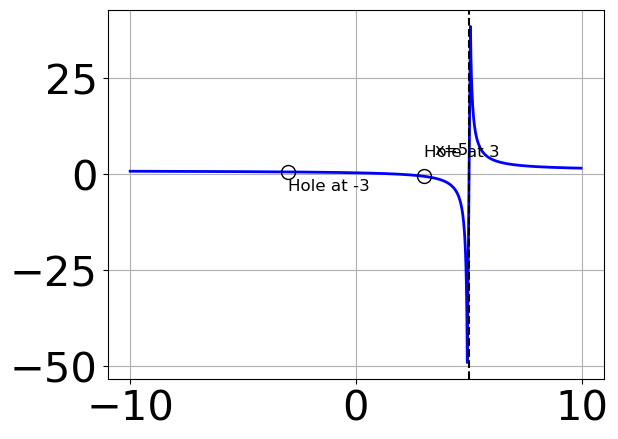
\includegraphics[width=0.5\textwidth]{../Figures/identifyGraphOfRationalFunctionA.png}
\end{center}
\begin{enumerate}[label=\Alph*.]
\item \( f(x)=\frac{x^{3} +7.0 x^{2} +4.0 x -12.0}{x^{3} +5.0 x^{2} -9.0 x -45.0} \)
\item \( f(x)=\frac{x^{3} +2.0 x^{2} -9.0 x -18.0}{x^{3} +5.0 x^{2} -9.0 x -45.0} \)
\item \( f(x)=\frac{x^{3} + x^{2} -16.0 x + 20.0}{x^{3} -5.0 x^{2} -9.0 x + 45.0} \)
\item \( f(x)=\frac{x^{3} -2.0 x^{2} -9.0 x + 18.0}{x^{3} -5.0 x^{2} -9.0 x + 45.0} \)
\item \( \text{None of the above are possible equations for the graph.} \)

\end{enumerate} }
\litem{
Determine the vertical asymptotes and holes in the rational function below.\[ f(x) = \frac{16x^{3} -72 x^{2} +17 x + 60}{8x^{2} -14 x -15} \]\begin{enumerate}[label=\Alph*.]
\item \( \text{Vertical Asymptotes of } x = 2.5 \text{ and } x = -0.75 \text{ with no holes.} \)
\item \( \text{Vertical Asymptotes of } x = 2.5 \text{ and } x = 1.25 \text{ with a hole at } x = -0.75 \)
\item \( \text{Vertical Asymptote of } x = 2.0 \text{ and hole at } x = -0.75 \)
\item \( \text{Vertical Asymptote of } x = 2.5 \text{ and hole at } x = -0.75 \)
\item \( \text{Holes at } x = 2.5 \text{ and } x = -0.75 \text{ with no vertical asymptotes.} \)

\end{enumerate} }
\litem{
Determine the horizontal and/or oblique asymptotes in the rational function below.\[ f(x) = \frac{5x^{2} -29 x + 20}{20x^{3} +49 x^{2} -112 x + 48} \]\begin{enumerate}[label=\Alph*.]
\item \( \text{Oblique Asymptote of } y = 4x + 33. \)
\item \( \text{Horizontal Asymptote of } y = 0 \)
\item \( \text{Horizontal Asymptote of } y = 0.250 \text{ and Oblique Asymptote of } y = 4x + 33 \)
\item \( \text{Horizontal Asymptote of } y = 0.250  \)
\item \( \text{Horizontal Asymptote at } y = 5.000 \)

\end{enumerate} }
\litem{
Determine the vertical asymptotes and holes in the rational function below.\[ f(x) = \frac{8x^{3} -6 x^{2} -45 x + 50}{12x^{2} +5 x -25} \]\begin{enumerate}[label=\Alph*.]
\item \( \text{Vertical Asymptote of } x = -1.667 \text{ and hole at } x = 1.25 \)
\item \( \text{Holes at } x = -1.667 \text{ and } x = 1.25 \text{ with no vertical asymptotes.} \)
\item \( \text{Vertical Asymptotes of } x = -1.667 \text{ and } x = -2.5 \text{ with a hole at } x = 1.25 \)
\item \( \text{Vertical Asymptote of } x = 0.667 \text{ and hole at } x = 1.25 \)
\item \( \text{Vertical Asymptotes of } x = -1.667 \text{ and } x = 1.25 \text{ with no holes.} \)

\end{enumerate} }
\litem{
Determine the horizontal and/or oblique asymptotes in the rational function below.\[ f(x) = \frac{6x^{3} +11 x^{2} -x -6}{2x^{2} +11 x + 12} \]\begin{enumerate}[label=\Alph*.]
\item \( \text{Horizontal Asymptote of } y = -4.0 \text{ and Oblique Asymptote of } y = 3x -11 \)
\item \( \text{Horizontal Asymptote of } y = 3.0 \text{ and Oblique Asymptote of } y = 3x -11 \)
\item \( \text{Horizontal Asymptote at } y = -4.0 \)
\item \( \text{Oblique Asymptote of } y = 3x -11. \)
\item \( \text{Horizontal Asymptote of } y = 3.0  \)

\end{enumerate} }
\litem{
Determine the horizontal and/or oblique asymptotes in the rational function below.\[ f(x) = \frac{6x^{3} -23 x^{2} -16 x + 48}{3x^{2} +8 x -16} \]\begin{enumerate}[label=\Alph*.]
\item \( \text{Horizontal Asymptote of } y = -4.0 \text{ and Oblique Asymptote of } y = 2x -13 \)
\item \( \text{Horizontal Asymptote at } y = -4.0 \)
\item \( \text{Horizontal Asymptote of } y = 2.0  \)
\item \( \text{Horizontal Asymptote of } y = 2.0 \text{ and Oblique Asymptote of } y = 2x -13 \)
\item \( \text{Oblique Asymptote of } y = 2x -13. \)

\end{enumerate} }
\end{enumerate}

\end{document}